
\newcounter{CTS} % Contatore Test
\newcommand{\stepCTS}[0]{\stepcounter{CTS}} % incrementa il contatore CTS
\newcommand{\valueCTS}[0]{\stepCTS TS\arabic{CTS}\label{_TS\arabic{CTS}}} % ritorna il valore del contatore CTS incrementato di 1
\newcommand{\refCTS}[0]{\stepCTS \hyperref[_TS\arabic{CTS}]{TS\arabic{CTS}}}
\newcommand{\resetCTS}[0]{\setcounter{CTS}{0}}
\resetCTS

\section{Strategia di testing} \label{_test}
La strategia di testing adottata dal gruppo è basata sul modello a V la quale stabilisce una stretta correlazione tra l'attività di testing prevista e la sua rispettiva attività nella parte sinistra \\
\begin{figure}[!htb]
	\centering
	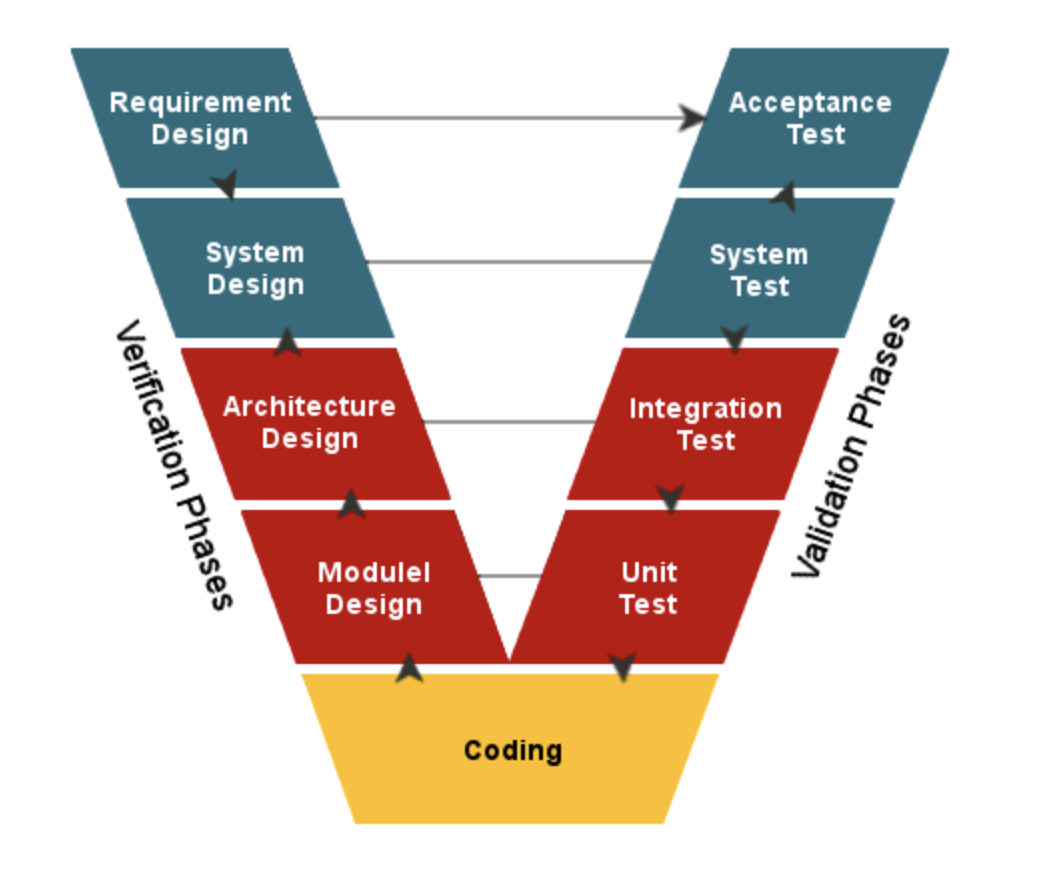
\includegraphics[scale=0.50]{res/images/vtestmodel.png}
	\caption{Modello a V}
\end{figure}

\subsection{Specifica dei test}
\begin{itemize}
	\item \textbf{Test di unità:} si effettua per verificare il corretto comportamento di un singolo componente del programma in modo indipendente da altre unità;
	\item \textbf{Test di integrazione:} si effettua per verificare la corretta integrazione tra due o più unità distinte;
	\item \textbf{Test di sistema:} verificano la funzionalità dell'interno sistema verificando il soddisfacimento dei requisiti obbligatori;
	\item \textbf{Test di accettazione:} vengono eseguiti in collaborazione con il committente prima di procedere al rilascio.
\end{itemize}

\subsection{Test di sistema} \label{_testSistema}
I test di sistema devono assicurare il soddisfacimento dei requisiti individuati nel documento \dext{AnalisiDeiRequisiti\_1.0.0}.
Di seguito l'elenco dei test di sistema individuati.

\newpage

\begin{center}
	\rowcolors{1}{white}{blue!20}
	\begin{longtable}{|p{1cm}|p{4.85cm}|p{9cm}|}
		\hline
		\rowcolor{lighter-grayer}
		\textbf{Codice} & \textbf{Titolo} & \textbf{Descrizione} \\
		\hline
		\endfirsthead
		\hline
		\multicolumn{3}{|c|}{\textit{Continua nella pagina successiva...}} \\
		\hline
		\endfoot
		\endlastfoot

		\hline
		
		\valueCTS & Visualizzazione homepage e carrello & Verificare che un utente generico possa:
		\begin{enumerate}
			\item  visualizzare la homepage ed i prodotti in evidenza in essa contenuti;
			\item  raggiungere e visualizzare la pagina del carrello da ogni pagina dell'applicativo.
		\end{enumerate} \\

		\valueCTS & Visualizzazione informazioni venditore & Verificare che un utente generico possa visualizzare la pagina contenente le informazioni relative al venditore che includono la ragione sociale e i contatti. \\

		\valueCTS & Funzionalità menù categorie & Verificare che un utente generico: 
		\begin{enumerate}
			\item  possa cliccare in una delle voci del menù delle categorie;
			\item  riceva un messaggio di errore se non vi sono prodotti all'interno della categoria selezionata.
		\end{enumerate} \\

		\valueCTS & Funzionalità ricerca & Verificare che un utente generico: 
		\begin{enumerate}
			\item  possa cercare un prodotto mediante il proprio nome utilizzando la funzionalità di ricerca;
			\item  riceva un messaggio di errore se non vi sono prodotti che soddisfano la \glock{query} di ricerca.
		\end{enumerate} \\

		\valueCTS & Visualizzazione \glock{PLP} & Verificare che un utente generico possa: 
		\begin{enumerate}
			\item  visualizzare una PLP;
			\item  visualizzare la lista prodotti con le relative immagini, titolo e prezzo IVA inclusa;
			\item  visualizzare la disponibilità o meno dei prodotti elencati;
			\item  cliccare in un prodotto per accedere alla relativa \glock{PDP}.
		\end{enumerate} \\

		\valueCTS & Ordinamento prodotti PLP & Verificare che un utente generico possa: 
		\begin{enumerate}
			\item  ordinare i prodotti della PLP per prezzo crescente o decrescente;
			\item  ordinare i prodotti della PLP per ordine alfabetico.
		\end{enumerate} \\

		\valueCTS & Filtri PLP & Verificare che un utente generico possa: 
		\begin{enumerate}
			\item  applicare, modificare e rimuovere uno o più filtri di visualizzazione prodotti basati su un prezzo minimo e/o massimo;
			\item  applicare, modificare e rimuovere uno o più filtri basati su una categoria;
			\item  visualizzare un messaggio di errore nel caso nessun prodotto soddisfi i filtri applicati.
		\end{enumerate} \\

		\valueCTS & Visualizzazione PDP & Verificare che un utente generico possa visualizzare: 
		\begin{enumerate}
			\item   la PDP di un prodotto contenente la descrizione ed una o più foto del prodotto;
			\item   la disponibilità o meno del prodotto;
			\item   il prezzo del prodotto IVA inclusa;
			\item   se ha già aggiunto l'articolo nel carrello.
		\end{enumerate} \\

		\valueCTS & Aggiunta a carrello & Verificare che un utente generico possa : 
		\begin{enumerate}
			\item   aggiungere un prodotto al carrello potendo specificare la quantità;
			\item   visualizzare un errore nel caso voglia aggiungere al carrello una quantità maggiore di quella disponibile.
		\end{enumerate} \\

		\valueCTS & Sincronizzazione carrello & Verificare che un utente autenticato possa recuperare il proprio carrello da qualsiasi dispositivo esso faccia il login.\\

		\valueCTS & Apertura pagina carrello & Verificare che: 
		\begin{enumerate}
			\item i prodotti inseriti precedentemente vengano visualizzati nella giusta quantità;
			\item il totale dell'ordine sia corretto (solo prodotti, senza tasse e spedizione);
			\item il totale dell'ordine con le tasse aggiunte sia corretto;
			\item si possa vedere il costo dei singoli prodotti;
			\item si visualizzi il messaggio di carrello vuoto nel caso in cui lo sia.
		\end{enumerate} \\

		\valueCTS & Modifica quantità prodotti nel carrello & Verificare che:
		\begin{enumerate}
			\item si possa aumentare e diminuire la quantità di un singolo articolo nel carrello;
			\item in caso di aumento, se la quantità richiesta non è disponibile, venga visualizzato il giusto messaggio di errore;
			\item si possa eliminare un singolo articolo.
		\end{enumerate}\\

		\valueCTS & Svuotare il carrello & Verificare che tutti gli elementi nel carrello possano essere rimossi. \\

		\valueCTS & Processo di checkout & Verificare che:
		\begin{enumerate}
			\item il messaggio mostri un errore se si avvia il checkout con carrello vuoto;
			\item si possano inserire indirizzi di fatturazione e spedizione da form e da quelli salvati (se autenticato);
			\item l'indirizzo di spedizione possa essere copiato con un click da quello scelto per la fatturazione;
			\item vengano aggiunti e visualizzati i costi di spedizione al totale dell'ordine, dopo aver scelto l'indirizzo di spedizione. 
			\item il sistema di pagamento con il provider esterno possa essere utilizzato per concludere il checkout;
			\item nel caso di fallimento del pagamento, il sistema mostri in modo chiaro che il pagamento non è andato a buon fine e l'ordine non è stato emesso;
			\item nel caso di fallimento del pagamento, si possa riprovare immediatamente;
			\item in caso di successo del pagamento, si avvisa il cliente dell'avvenuto ordine, vengono scalate le merci acquistate dal magazzino e il venditore possa gestire l'ordine.
		\end{enumerate} \\

		\valueCTS & Login cliente & Verificare che:
		\begin{enumerate}
			\item il sistema di login cliente permetta di autenticarsi all'applicazione con un profilo già registrato, inserendo le corrette credenziali;
			\item il cliente possa navigare tutto il sito mantenendo la sessione di login;
			\item in caso di credenziali errate, venga mostrato il relativo messaggio di errore e si permetta di riprovare nell'immediato.
		\end{enumerate} \\

		\valueCTS & Registrazione cliente & Verificare che:
		\begin{enumerate}
			\item un cliente non autenticato possa avviare il processo di registrazione;
			\item nel caso in cui il doppio inserimento dell'email fallisca (e.g. non corrisponde) si visualizzi il relativo messaggio d'errore;
			\item nel caso in cui il doppio inserimento della password fallisca (e.g. non corrisponde) si visualizzi il relativo messaggio d'errore;
			\item nel caso in cui la password non rispetti i requisiti minimi di sicurezza si visualizzi il relativo messaggio d'errore;
			\item nel caso in cui esista già un utente con la stessa email si visualizzi il relativo messaggio d'errore;
			\item nel caso in cui tutto vada a buon fine, arrivi l'email per la verifica dell'indirizzo inserito;
			\item il click sul link di conferma ricevuto abiliti l'account appena registrato.
		\end{enumerate} \\

		\valueCTS & Recupero password cliente & Verificare che:
		\begin{enumerate}
			\item durante il processo di login si possa avviare quello per il recupero della password;
			\item si riceva il link per la reimpostazione della password al proprio indirizzo email, nel caso si richieda;
			\item cliccando il link ricevuto si possa inserire la password con un doppio inserimento;
			\item nel caso in cui i due inserimenti non corrispondano e/o la password non rispetti i requisiti di sicurezza si mostri il relativo messaggio d'errore;
			\item nel caso in cui si inseriscano dei dati validi, mostrare il messaggio di conferma cambio password.
		\end{enumerate} \\

		\valueCTS & Amministrazione account cliente - gestione indirizzi & Verificare che:
		\begin{enumerate}
			\item si possa inserire un nuovo indirizzo e che questo sia utilizzabile durante il processo di checkout; 
			\item nel caso in cui si inserisca un indirizzo non valido (e.g. campi obbligatori vuoti) si mostri un messaggio di errore e si permetta la modifica immediata dei dati inseriti;
			\item si possa eliminare un indirizzo precedentemente inserito.
		\end{enumerate} \\

		\valueCTS & Amministrazione account cliente - assistenza & Verificare che:
		\begin{enumerate}
			\item il cliente possa aprire un ticket di assistenza e che questo sia gestibile dal venditore;
			\item il cliente possa avviare la richiesta di cancellazione account tramite un apposito tipo di ticket di assistenza.
		\end{enumerate} \\

		\valueCTS & Amministrazione account cliente - modifica dati login & Verificare che:
		\begin{enumerate}
			\item il cliente possa cambiare indirizzo email;
			\item il sistema si comporti per il cambio email come nel processo di registrazione;
			\item il cliente possa cambiare password inserendo quella vecchia;
			\item il sistema si comporti per il cambio password come nel processo di registrazione. 
		\end{enumerate} \\

		\valueCTS & Verifica gestione propri ordini & Verificare che:
		\begin{enumerate}
			\item il cliente possa gestire i propri ordini;
			\item il cliente possa contattare il venditore tramite i form per:
			\begin{enumerate}
				\item annullare l'ordine;
				\item segnalare problemi dell'ordine;
				\item chiedere il reso.
			\end{enumerate}
		\end{enumerate} \\

		\valueCTS & Verifica logout cliente & Verificare che il cliente loggato possa effettuare il logout e che venga riportato alla home page \\

		\valueCTS & Verifica contatto venditore & Verificare che il cliente possa contattare il venditore tramite l'apposito form  \\

		\valueCTS & Verifica dashboard ordini venditore & Verificare che:
		\begin{enumerate}
			\item il venditore possa visualizzare e modificare la lista degli ordini ricevuti;
			\item il venditore possa cercare un ordine presente nel sistema;
			\item il venditore possa ordinare gli ordini presenti nel sistema;
			\item il venditore possa modificare lo stato di un ordine;
			\item il venditore possa stampare la bolla per un ordine;
			\item il venditore possa visualizzare i dettagli di un ordine;
		\end{enumerate} \\

		\valueCTS & Verifica dashboard clienti venditore & Verificare che:
		\begin{enumerate}
			\item il venditore possa visualizzare la lista dei clienti;
			\item il venditore possa cercare un determinato cliente nel sistema;
			\item il venditore possa ordinare i clienti con determinati filtri;
			\item il venditore possa contattare il cliente tramite un form.
		\end{enumerate} \\

		\valueCTS & Verifica dashboard aliquote venditore & Verificare che:
		\begin{enumerate}
			\item il venditore possa gestire le aliquote IVA per la tassazione dei prodotti;
			\item il venditore possa visualizzare le aliquote IVA già presenti nel sistema;
			\item il venditore possa aggiungere un'aliquota IVA;
			\item il venditore possa modificare un'aliquota IVA;
			\item il venditore possa eliminare un'aliquota IVA già presente nel sistema.
		\end{enumerate} \\

		\valueCTS & Verifica dashboard prodotti venditore & Verificare che:
		\begin{enumerate}
			\item il venditore possa visualizzare la lista dei prodotti inseriti nel sistema;
			\item il venditore possa cercare un prodotto presente nel sistema;
			\item il venditore possa filtrare i prodotti;
			\item il venditore possa aggiungere un prodotto al sistema dopo aver compilato tutti i campi obbligatori del prodotto;
			\item il venditore possa modificare un prodotto aggiornando i campi già presenti;
			\item il venditore possa eliminare un prodotto presente nel sistema;
			\item il venditore possa selezionare i prodotti da mostrare nella HomePage cliente.
		\end{enumerate} \\

		\valueCTS & Verifica dashboard categorie venditore & Verificare che:
		\begin{enumerate}
			\item il venditore possa visualizzare tutte le categorie presenti nel sistema;
			\item il venditore possa aggiungere una categoria di prodotti impostando il nome;
			\item il venditore possa rimuovere una categoria di prodotti;
			\item il venditore possa modificare il nome di una categoria già esistente nel sistema.
		\end{enumerate} \\

		\valueCTS & Verifica login venditore & Verificare che il venditore possa effettuare il login \\

		\valueCTS & Verifica login venditore & Verificare che il venditore possa effettuare il logout \\

		\hline
		\caption{Test di sistema}
	\end{longtable}
\end{center}


\subsection{Tracciamento test di sistema - requisiti}
La seguente tabella riporta l'associazione dei test precedentemente descritti con i requisiti presenti nel documento \dext{AnalisiDeiREquisiti\_1.0.0}. Si precisa che ogni test comprende anche eventuali sotto requisiti.
\resetCTS
\begin{center}
	\rowcolors{1}{white}{blue!20}
	\begin{longtable}{|c|c|}
		\hline
		\rowcolor{lighter-grayer}
		\textbf{Test di sistema} & \textbf{Requisiti} \\
		\hline
		\endfirsthead
		\hline
		\multicolumn{2}{|c|}{\textit{Continua nella pagina successiva...}} \\
		\hline
		\endfoot
		\endlastfoot

		\hline
		\refCTS & R1F1 \\
		\refCTS & R1F2 \\
		\refCTS & R1F3 \\
		\refCTS & R1F4 \\
		\refCTS & R1F5 \\
		\refCTS & R2F6 \\
		\refCTS & R1F7 \\
		\refCTS & R1F8 \\
		\refCTS & R1F9 \\
		\refCTS & R1F10 \\

		\refCTS & R1F11  \\
		\refCTS & R1F12 \\
		\refCTS & R3F13 \\
		\refCTS & R1F14 \\
		\refCTS & R1F15 \\
		\refCTS & R1F16 \\
		\refCTS & R1F17 \\
		\refCTS & R1F18 \\
		\refCTS & R1F18 \\
		\refCTS & R1F18 \\

		\refCTS & R1F19 \\
		\refCTS & R1F20 \\
		\refCTS & R1F21 \\
		\refCTS & R1F22 \\
		\refCTS & R1F23 \\
		\refCTS & R1F24 \\
		\refCTS & R1F25 \\
		\refCTS & R1F26 \\
		\refCTS & R1F27 \\
		\refCTS & R1F28 \\
		
		\hline
		\caption{Tracciamento test di sistema - requisiti}
	\end{longtable}
\end{center}



